
% NE PAS TOUCHER
%++++++++++++++++++++++++++++++++++++++++
\documentclass[letterpaper,12pt]{article}
\usepackage{tabularx}
\usepackage{amsmath}
\usepackage{graphicx}
\usepackage[margin=1in,letterpaper]{geometry}
\usepackage{cite}
\usepackage[final]{hyperref}
\usepackage{datatool}
\usepackage{caption}
\usepackage{float}
\usepackage{gensymb}

\hypersetup{
	colorlinks=true,
	linkcolor=blue,
	citecolor=blue,
	filecolor=magenta,
	urlcolor=blue
}
%+++++++++++++++++++++++++++++++++++++++++

%	INCLUDES
\graphicspath{ {./ressources/images} }

\begin{document}

\title{Automatique}

\author{Seite Alexander et Nathan Vidonne}
\date{\today}
\maketitle
\newline

\tableofcontents

\newpage

%%%%%%%%%%%%%%%%%%%%%%%%%%%%%%%%%%%%
%	Intro 
%%%%%%%%%%%%%%%%%%%%%%%%%%%%%%%%%%%%
\section{Introduction}
Dans ce rapport, nous etudions le comportement d'un banc de tesst SIRAu. Il s'agit d'un motoreducteur instrumenté constitué donc d'un moteur à courant continu avec réducteur et génératrice tachymétrique. Ce dernier est piloté par un contrôleur de chez Maxon dont on ne dispose pas la référence du modèle.
\\
Nous analysons en deux temps ce banc de test. D'abord, nous discutons par des représentations graphiques le comportement du banc de test à partir de données empiriques qui nous a permi de charactériser la fonction de transfert du modèle. Cette dernière nous permit en un second temps d'analyser la stabilité du système asservi. Nous comparerons les résultats représentés par les différentes méthodes de manière à être en mesure d’établir un lien entre elles.
\\
Par conséquent, les objectifs sont de faire le lien entre un comportement mesuré sur une installation réelle et une représentation par fonction de transfert et de comprendre et expliciter ce que l’on peut observer sur les représentations graphiques usuelles (Bode, Nyquist, Evans. Ref.\cite{protocole} 
\\
La completion de ces objectifs permettrons de nous familiariser avec les commandes MATLAB pour afficher ces graphs au travers l'utilisation de l'app "Control system designer et l'analyse des résultats. \\
%%%%%%%%%%%%%%%%%%%%%%%%%%%%%%%%%%%%
%	Exercices 
%%%%%%%%%%%%%%%%%%%%%%%%%%%%%%%%%%%%
\section{Exercice 1 : Analyse empirique du banc de test}


\begin{figure}[H]
    \begin{center}
        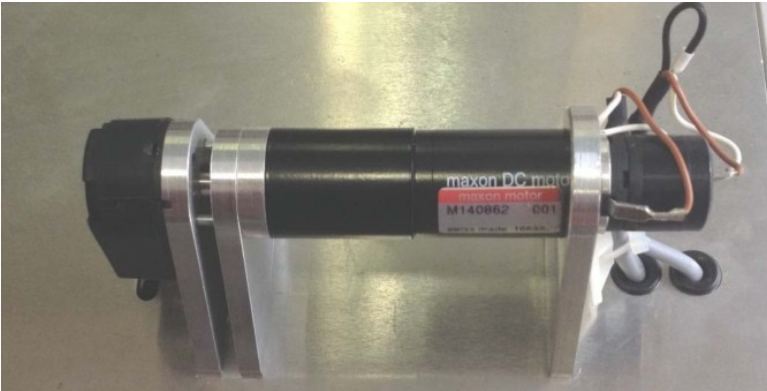
\includegraphics[width=\textwidth]{test.png}
    \label{fig:test}
    \end{center}
\end{figure}

\hspace{1cm}

\vspace{1cm}


\subsection{A : Estimation de la fonction de transfert du système}

%Estimation simple du systeme
Pour le gain estime de k = 85 et une constante de temps tau = 0.01, nous retrouvons un système du premier ordre : 

\[
    G(s) = \frac{K}{1 + \tau \cdot s}
\]

\subsection{B/C/D : Vérification de la fonction de transfert}

Dans le graphique suivant, nous pouvons observer que nous avons dû rajouter un retard de 0.1s afin de pouvoir comparer les données mesurées (bleu) et la courbe théorique (rouge).

\begin{figure}[H]
    \begin{center}
    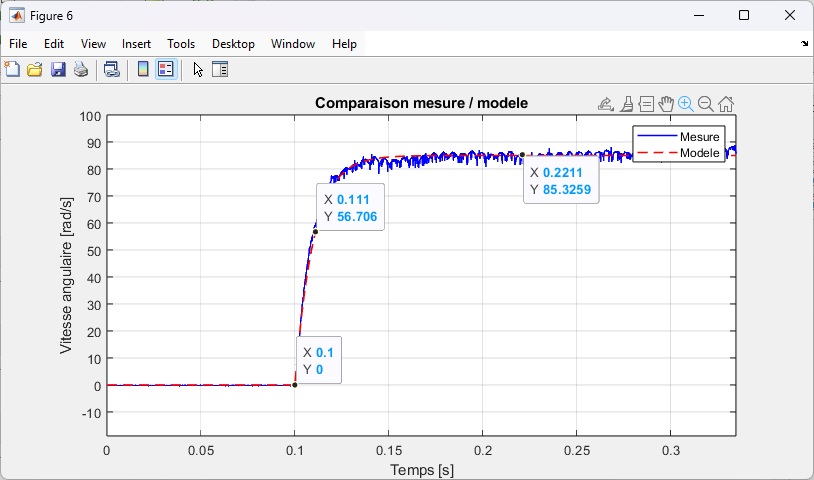
\includegraphics[scale=0.8]{FIG_A_propre.png}
    \label{fig:}
    \end{center}
\end{figure}

Par définition, $\tau$ peut être déterminé à 66\% du gain final. Nous trouvons 0.111. Cela n'est pas egal a la valeur theorique, mais cela s'explique par le fait que nous ayons ajoute un retard de 0.1. Comme 0.111 - 0.1 = 0.011, nous trouvons en effet une valeurs proche du modele pour $\tau$. Le gains statique qu'illustre Fig. \ref{fig:A} est lui aussi proche de la valeur theorique (85.3259 $\approx$ 85). 

\newpage


%%%%%%%%%%%%%%%%%%%%%%%%%%%%%%%%%%%%
%       Exercices 
%%%%%%%%%%%%%%%%%%%%%%%%%%%%%%%%%%%%

\section{Exercice 2 : Rentrons bien dans les details}

Nous schematisons notre systeme sur Fig. \ref{fig:graph} par le produit de 3 sous-systemes (moteur, mesure, element) \cite{protocole}.
\begin{figure}[H]
        \begin{center}
        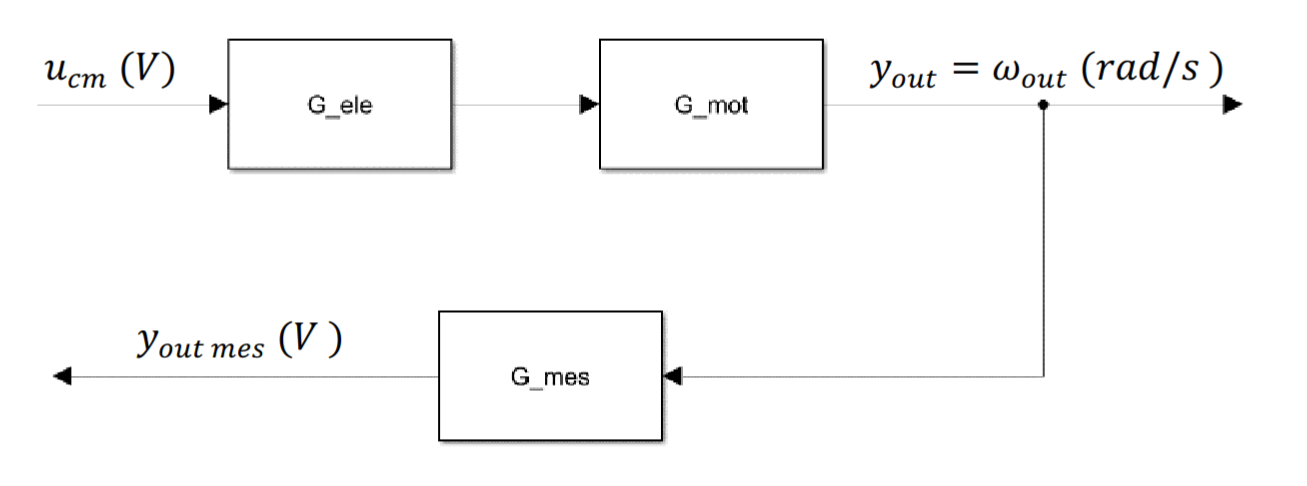
\includegraphics[scale=0.4]{graph.png}
            \label{fig:graph}
        \end{center}
\end{figure}
Les fonctions de transfert des sous systemes sont respectivement :
\[
    G_m_o_t(s) = \frac{4.53 \cdot 10^3}{1 + s\cdot 8 \cdot 10^-3}
\]
\[
    G_e_l_e(s) = \frac{20.8 \cdot 10^-3}{1 + s\cdot 1.5 \cdot 10^-4}
\]
\[
    G_m_e_s(s) = 10.7 \cdot 10^-3
\]


\subsection{A : Verification graphique}
\label{sec:A}
\begin{figure}[H]
        \begin{center}
            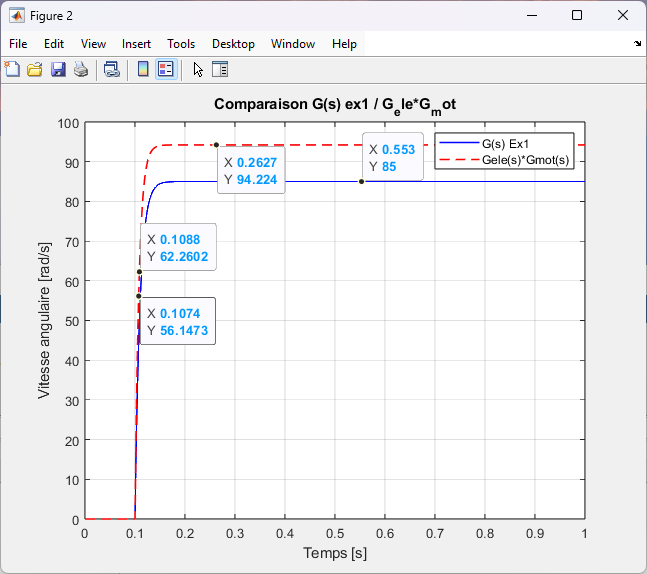
\includegraphics[scale=0.8]{FIG_A_exercice2.png}
        \end{center}
\end{figure}

\\\\
Nous constatons que les deux courbes ne sont pas identiques et que le gain change. Elles restent tout de meme similaires.
\\(Comme le titre est illisible, nous pensions a : "Comparaison entre G(s) / $G_e_l_e$ * $G_m_o_t$")
\newpage
\subsection{B : Fonction de transfert du systeme complet}

Nous etablissons la fonction de transfert a partir de $G_m_o_t$ * $G_e_l_e$ * $G_m_e_s$ tel que : 
\begin{figure}[H]
	\begin{center}
	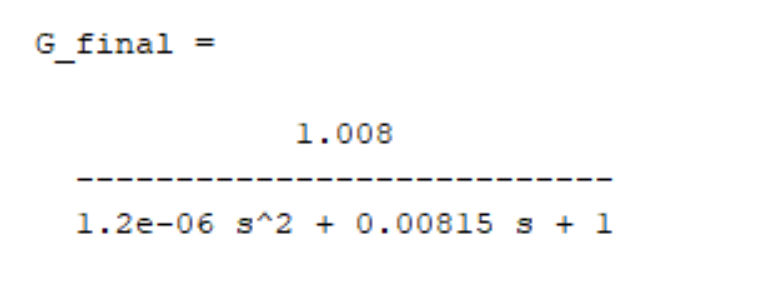
\includegraphics[scale=0.55]{GS.png}
	\end{center}
\end{figure}
\begin{figure}[H]
        \begin{center}
                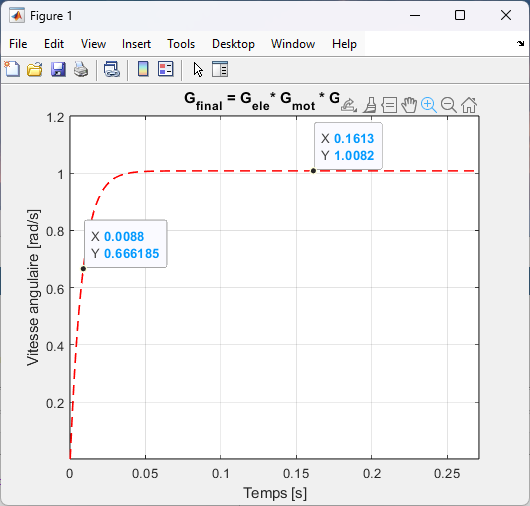
\includegraphics[scale=0.8]{FIG_B_ex2.png}
                    \end{center}
\end{figure}

%\vspace{1cm}
%\noindent \begin{minipage}{0.45\textwidth}
%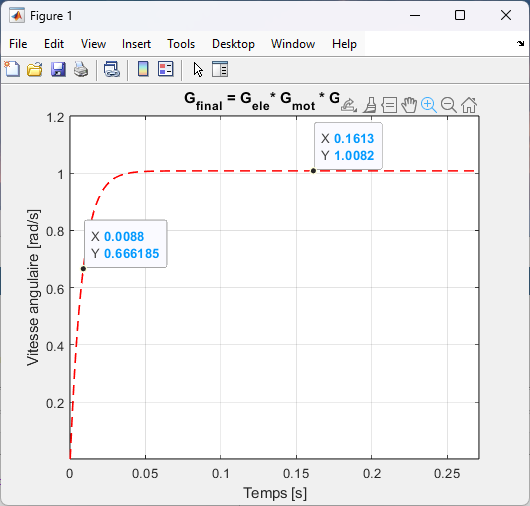
\includegraphics[width=\textwidth]{FIG_B_ex2.png}
%\end{minipage}
%\hspace{1cm}
%\begin{minipage}{0.45\textwidth}
%    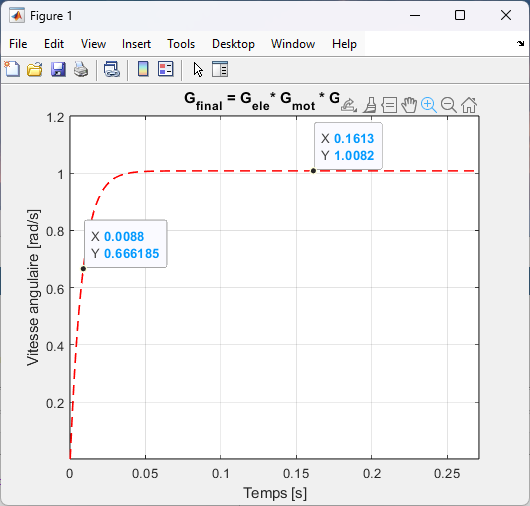
\includegraphics[width=\textwidth]{FIG_B_ex2.png}
%\noindent 
%\end{minipage}

\vspace{1cm}
(Nous avons compris entre temps comment avoir de jolis titres)

\newpage

\subsection{C : Code definissant la fonction de transfert}
load('/MT/systeme/asservis/SIRAu/stepResponse.mat')
\\
t = time;
\\
\\clear; close all; clc;
\\
\\s = tf('s');
\\
\\K\_mot = 4.53e3;
\\tau\_mot = 8e-3;
\\G\_mot = K\_mot / (1 + tau\_mot*s);
\\K\_ele = 20.8e-3;
\\tau\_ele = 1.5e-4;
\\G\_ele = K\_ele / (1 + tau\_ele*s);
\\K\_mes = 10.7e-3;
\\G\_mes = tf(K\_mes);
\\G\_final = G\_mot * G\_ele * G\_mes;
\\\%disp('===== G\_s =====')
\\G\_final


\newpage
\subsection{D : Application d'un regulateur PI}

\begin{figure}[H]
        \begin{center}
                
\includegraphics[scale=0.6]{Exo2_B_scop.png}
                    \end{center}
\end{figure}


\subsection{E : Diagrammes de Bode et Nyquist}

Montrer marge de phase... (completer)
\begin{figure}[H]
        \begin{center}
                
\includegraphics[scale=0.6]{Exo2_B_scop.png}
                    \end{center}
\end{figure}


\subsection{F : Diagramme d'Evans et reponse indicielle}

\begin{figure}[H]
        \begin{center}
                
\includegraphics[scale=0.6]{Exo2_B_scop.png}
                    \end{center}
\end{figure}


\subsection{G : G(s) dans "Control System Designer"}

\begin{figure}[H]
        \begin{center}
                
\includegraphics[scale=0.6]{Exo2_B_scop.png}
                    \end{center}
\end{figure}

\subsection{H : (MATLAB == CSD) ? verification graphique}

\begin{figure}[H]
        \begin{center}
                
\includegraphics[scale=0.6]{Exo2_B_scop.png}
                    \end{center}
\end{figure}

\subsection{I : Marges de stabilite sur diagramme de Bode}

\begin{figure}[H]
        \begin{center}
                
\includegraphics[scale=0.6]{Exo2_B_scop.png}
                    \end{center}
\end{figure}

\subsection{J : Lieu des poles (vous nous avez dit de passer cette question)}
s
%\begin{figure}[H]
%        \begin{center}
%                
\includegraphics[scale=0.6]{Exo2_B_scop.png}
%                    \end{center}
%\end{figure}

\subsection{K : Caracteristiques de la reponse indicielle}

\begin{figure}[H]
        \begin{center}
                
\includegraphics[scale=0.6]{Exo2_B_scop.png}
                    \end{center}
\end{figure}

\subsection{L : Lien entre gain du regulateur et valeurs de depassement}

\begin{figure}[H]
        \begin{center}
                
\includegraphics[scale=0.6]{Exo2_B_scop.png}
                    \end{center}
\end{figure}

\subsection{M : Impact du gain sur la stabilite du systeme}

\begin{figure}[H]
        \begin{center}
                
\includegraphics[scale=0.6]{Exo2_B_scop.png}
                    \end{center}
\end{figure}


\newpage


%%%%%%%%%%%%%%%%%%%%%%%%%%%%%%%%%%%%
%       Conclusion 
%%%%%%%%%%%%%%%%%%%%%%%%%%%%%%%%%%%%
\section{Conclusion}
\begin{figure}[H]
        \begin{center}
        
\includegraphics[scale=0.45]{all.png}
        \end{center}
\end{figure}
\begin{figure}[H]
\begin{center}
        
\includegraphics[scale=0.4]{all_graph.png}
\end{center}
\end{figure}


\newpage
\section{annexes}
\end{document}


